\documentclass[aspectratio=169, table, xcdraw]{beamer}

% Tema y Colores Institucionales
\usetheme{Madrid}
\usecolortheme{default}
\definecolor{ucbblue}{RGB}{0, 51, 102}

% Ajuste de contrastes
\setbeamercolor{structure}{fg=ucbblue}
\setbeamercolor*{palette primary}{fg=white,bg=ucbblue}
\setbeamercolor*{palette secondary}{fg=white,bg=ucbblue!80}
\setbeamercolor*{palette tertiary}{fg=white,bg=ucbblue!90}
\setbeamercolor{title}{fg=white, bg=ucbblue}
\setbeamercolor{frametitle}{fg=white, bg=ucbblue}
\setbeamercolor{item}{fg=ucbblue}

% Fuentes, Matemáticas e Idioma (Configuración a prueba de fallos)
\usepackage[T1]{fontenc}
\usepackage[utf8]{inputenc}
\usepackage{tgpagella}
\usefonttheme{serif} % OBLIGATORIO: Fuerza a Beamer a usar la fuente Pagella
\usepackage[spanish, es-noshorthands]{babel}
\renewcommand{\tablename}{Tabla}
\renewcommand{\figurename}{Figura}

\usepackage{amsmath, amssymb, bm}
\usepackage{graphicx}
\usepackage{booktabs}
\usepackage[most]{tcolorbox} % SOLUCIÓN: Paquete faltante para el Exit Check

% TikZ (Completamente saneado)
\usepackage{tikz}
\usetikzlibrary{shapes.geometric, arrows.meta, positioning, calc}

% Configuración para código fuente (XML/URDF)
\usepackage{listings}
\lstset{
    basicstyle=\ttfamily\tiny, % Reducido a \tiny para evitar Overfull \vbox
    backgroundcolor=\color{gray!10},
    frame=single,
    rulecolor=\color{gray!40},
    keywordstyle=\color{blue}\bfseries,
    stringstyle=\color{red!70!black},
    commentstyle=\color{green!60!black},
    showstringspaces=false,
    morekeywords={robot, link, joint, origin, axis, parent, child, limit}
}

% Información del documento
\title[ABB IRB 120: D-H y URDF]{Modelado Cinemático del ABB IRB 120}
\subtitle{De la Convención D-H a la Descripción URDF en ROS}
\author[B. Quiroga Turdera]{M.Sc. Ing. Bernardo Quiroga Turdera}
\institute[UCB Tarija]{Universidad Católica Boliviana ``San Pablo'' — Sede Tarija \\ Robótica (IMT-342)}
\date{Jueves, 27 de Agosto de 2026}

\begin{document}

\begin{frame}
    \titlepage
\end{frame}

% =================================================================
% PARTE 1: OPENING CHALLENGE
% =================================================================
\begin{frame}{El Desafío de Hoy}
    \begin{center}
        \large \textit{¿Cómo transformamos un mecanismo físico de metal y motores en un modelo matemático y computacional que ROS pueda controlar?}
    \end{center}
    
    \vspace{0.4cm}
    \begin{center}
    \begin{tikzpicture}[
        node distance=0.8cm and 1cm,
        box/.style={rectangle, draw=ucbblue, thick, fill=ucbblue!5, text width=3.5cm, align=center, rounded corners, minimum height=1.2cm},
        arrow/.style={-Stealth, thick, ucbblue, line width=1.5pt}
    ]
        \node[box] (robot) {\textbf{1. Robot Físico}\\(ABB IRB 120)\\ \footnotesize Eslabones y Juntas};
        \node[box, right=of robot] (math) {\textbf{2. Modelo Matemático}\\(Convención D-H)\\ \footnotesize Matrices y $SE(3)$};
        \node[box, right=of math] (ros) {\textbf{3. Modelo ROS}\\(URDF / XML)\\ \footnotesize Árbol Cinemático};
        
        \draw[arrow] (robot) -- (math);
        \draw[arrow] (math) -- (ros);
    \end{tikzpicture}
    \end{center}
    
    \vspace{0.3cm}
    \textbf{Identificación en el Laboratorio:}
    \begin{itemize}
        \item 6 articulaciones de revolución (J1 a J6).
        \item Ejes de rotación ortogonales y paralelos.
        \item Marco base (inercial) vs. Marco de la herramienta (Brida/TCP).
    \end{itemize}
\end{frame}

% =================================================================
% PARTE 2: FRAME ASSIGNMENT
% =================================================================
\begin{frame}{Asignación de Marcos de Referencia (D-H Estándar)}
    \begin{columns}[T]
        \begin{column}{0.4\textwidth}
            \textbf{Repaso Rápido de Reglas:}
            \begin{enumerate}
                \item $z_{i-1}$ a lo largo del eje de la junta $i$.
                \item $x_i$ a lo largo de la perpendicular común ($z_{i-1} \to z_i$).
                \item Origen $O_i$ en la intersección de $x_i$ y $z_i$.
                \item $y_i$ completa la mano derecha.
            \end{enumerate}
        \end{column}
        
        \begin{column}{0.6\textwidth}
            \centering
            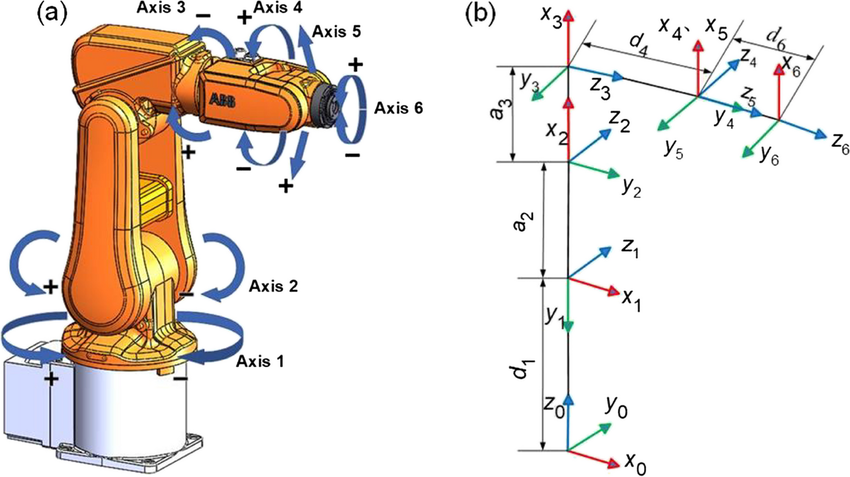
\includegraphics[width=0.8\textwidth]{../03_imagenes/dh_abb_irb_120.png}
        \end{column}
    \end{columns}
\end{frame}

% =================================================================
% PARTE 3: D-H TABLE & MATRICES
% =================================================================
\begin{frame}{Construcción de la Tabla D-H del ABB IRB 120}
    \begin{columns}[T]
        \begin{column}{0.5\textwidth}
            \textbf{Tabla de Parámetros Geométricos}
            \vspace{0.2cm}
            \begin{table}[]
                \centering
                \renewcommand{\arraystretch}{1.2}
                \begin{tabular}{c|c|c|c|c}
                \toprule
                $i$ & $\theta_i$ & $d_i$ & $a_i$ & $\alpha_i$ \\ \midrule
                1 & $q_1^*$ & [VALOR] & [VALOR] & [VALOR] \\
                2 & $q_2^*$ & [VALOR] & [VALOR] & [VALOR] \\
                3 & $q_3^*$ & [VALOR] & [VALOR] & [VALOR] \\
                4 & $q_4^*$ & [VALOR] & [VALOR] & [VALOR] \\
                5 & $q_5^*$ & [VALOR] & [VALOR] & [VALOR] \\
                6 & $q_6^*$ & [VALOR] & [VALOR] & [VALOR] \\ \bottomrule
                \end{tabular}
            \end{table}
            \footnotesize \textit{* $q_i$ representa la variable de articulación.} \\
            \footnotesize \textbf{Nota:} Utilizar cotas exactas del manual ABB.
        \end{column}
        
        \begin{column}{0.5\textwidth}
            \textbf{Composición Cinemática ($SE(3)$):} \\
            Cada fila produce una matriz homogénea:
            \small
            \begin{equation*}
                ^{i-1}T_i = R_z(\theta_i) T_z(d_i) T_x(a_i) R_x(\alpha_i)
            \end{equation*}
            \normalsize
            
            \vspace{0.2cm}
            \textbf{Cinemática Directa Total:} \\
            El encadenamiento ubica la brida del robot respecto a su base:
            \begin{equation*}
                ^0T_6 = {}^0T_1 \cdot {}^1T_2 \cdot {}^2T_3 \cdot {}^3T_4 \cdot {}^4T_5 \cdot {}^5T_6
            \end{equation*}
        \end{column}
    \end{columns}
\end{frame}

% =================================================================
% PARTE 4: D-H IS NOT URDF
% =================================================================
\begin{frame}{Conflicto Conceptual: D-H \textbf{no} es URDF}
    \vspace{-0.1cm}
    \begin{alertblock}{Precaución Estructural}
        Una fila de la tabla D-H \textbf{NO} se puede copiar y pegar directamente dentro del tag \texttt{<origin xyz="..." rpy="...">} de un archivo URDF. Cumplen propósitos matemáticos distintos.
    \end{alertblock}
    
    \vspace{0.1cm}
    \begin{center}
        \renewcommand{\arraystretch}{1.1}
        \resizebox{0.95\textwidth}{!}{
        \begin{tabular}{p{3.5cm} p{5.5cm} p{5.5cm}}
        \toprule
        \textbf{Atributo} & \textbf{Denavit-Hartenberg (D-H)} & \textbf{URDF (Unified Robot Desc. Format)} \\ \midrule
        \textbf{Parametrización} & Restringida a 4 parámetros ($z, x$) & Libre en $SE(3)$ (Transformación de 6 GDL) \\
        \textbf{Árbol Cinemático} & Implícito en la tabla (secuencial) & Explícito mediante tags \texttt{<parent>} / \texttt{<child>} \\
        \textbf{Mallas Visuales 3D} & No aplicable (puramente matemático) & Sí (Carga archivos \texttt{.stl} / \texttt{.dae}) \\
        \textbf{Límites y Físicas} & No definidos & Incorpora inercia, límites de torque, colisiones \\
        \textbf{Ecosistema} & Cálculo de Cin. Directa/Inversa & RViz, Gazebo, MoveIt! (ROS) \\ \bottomrule
        \end{tabular}
        }
    \end{center}
\end{frame}

% =================================================================
% PARTE 5: MINIMAL URDF
% =================================================================
\begin{frame}[fragile]{Estructura Mínima de URDF en ROS}
\vspace{-0.1cm}
\begin{lstlisting}[language=XML]
<robot name="irb120">
  <link name="base_link"/>
  <link name="link_1"/>

  <joint name="joint_1" type="revolute">
    <parent link="base_link"/>
    <child link="link_1"/>

    <!-- Transformacion del origen de J1 respecto a base_link -->
    <origin xyz="[VALOR_X] [VALOR_Y] [VALOR_Z]" rpy="0 0 0"/>
    
    <!-- Eje de rotacion de la articulacion en su propio marco local -->
    <axis xyz="0 0 1"/>

    <limit lower="[VALOR_MIN]" upper="[VALOR_MAX]" 
           effort="[TORQUE_MAX]" velocity="[VEL_MAX]"/>
  </joint>
  <!-- ... Eslabones subsecuentes ... -->
</robot>
\end{lstlisting}
\end{frame}

% =================================================================
% PARTE 6: CONCEPTUAL MAPPING
% =================================================================
\begin{frame}{Mapeo Conceptual: D-H $\rightarrow$ URDF}
    \textbf{Relación entre Dominios:} \\
    Aunque no hay conversión sintáctica 1:1, los conceptos físicos se mapean de la siguiente forma:
    
    \vspace{0.4cm}
    \begin{center}
    \begin{tikzpicture}[
        node distance=0.4cm and 2.5cm,
        box/.style={rectangle, draw=black, thick, fill=gray!10, text width=4.5cm, align=center, rounded corners},
        arrow/.style={-Stealth, thick, dashed, ucbblue}
    ]
        % D-H Side
        \node[box] (dh1) {Eje de Rotación Físico ($z_{i-1}$)};
        \node[box, below=of dh1] (dh2) {Geometría Relativa del Eslabón};
        \node[box, below=of dh2] (dh3) {Transformaciones $^{i-1}T_i$};
        \node[box, below=of dh3] (dh4) {Variable $q_i$ (Ángulo)};
        
        % URDF Side
        \node[box, fill=ucbblue!10, right=of dh1] (u1) {Vector \texttt{<axis xyz="..."/>}};
        \node[box, fill=ucbblue!10, right=of dh2] (u2) {Etiqueta \texttt{<origin xyz="..." rpy="..."/>}};
        \node[box, fill=ucbblue!10, right=of dh3] (u3) {Árbol de ROS (TF) / \texttt{parent}-\texttt{child}};
        \node[box, fill=ucbblue!10, right=of dh4] (u4) {\texttt{<joint type="revolute">}};

        % Arrows
        \draw[arrow] (dh1) -- (u1);
        \draw[arrow] (dh2) -- (u2);
        \draw[arrow] (dh3) -- (u3);
        \draw[arrow] (dh4) -- (u4);
    \end{tikzpicture}
    \end{center}
\end{frame}

% =================================================================
% PARTE 7: LABORATORY ACTIVITY
% =================================================================
\begin{frame}[fragile]{Actividad de Laboratorio: Implementación URDF}
    \begin{columns}[T]
        \begin{column}{0.4\textwidth}
            \textbf{Estructura del Paquete ROS:}
\begin{lstlisting}[basicstyle=\ttfamily\tiny, backgroundcolor=\color{white}]
irb120_description/
|-- package.xml
|-- CMakeLists.txt
|-- urdf/
|   `-- irb120.urdf
|-- meshes/
|   |-- visual/
|   `-- collision/
`-- launch/
    `-- display.launch
\end{lstlisting}
        \end{column}
        
        \begin{column}{0.6\textwidth}
            \textbf{Objetivo:} Implementar la cadena cinemática del ABB IRB 120. \\
            \vspace{0.3cm}
            \textbf{Puertas de Verificación (Checkpoints):}
            \begin{itemize}
                \item[$\square$] El XML es válido (usar \texttt{check\_urdf}).
                \item[$\square$] El árbol Parent-Child es secuencial.
                \item[$\square$] Las 6 articulaciones revolucionan en el eje físico correcto al variar el \textit{Joint State Publisher}.
                \item[$\square$] Los límites coinciden con el manual ABB.
            \end{itemize}
            \vspace{0.2cm}
            \textit{\textbf{Prioridad:} Estructura cinemática > Aspecto visual de mallas STL.}
        \end{column}
    \end{columns}
\end{frame}

% =================================================================
% PARTE 8: PREPARATION FOR EC1
% =================================================================
\begin{frame}{El Camino hacia el Hito 1 (Evaluación EC1)}
    \begin{center}
    \begin{tikzpicture}[
        node distance=1.5cm,
        box/.style={rectangle, draw=ucbblue, thick, fill=white, text width=2.8cm, align=center, rounded corners, minimum height=1cm, font=\scriptsize},
        arrow/.style={-Stealth, thick, ucbblue}
    ]
        \node[box] (f1) {\textbf{1.} Asignación de Marcos D-H};
        \node[box, right=of f1] (f2) {\textbf{2.} Tabla D-H y Matrices $T$};
        \node[box, right=of f2] (f3) {\textbf{3.} Cinemática Directa Numérica};
        \node[box, below=of f3] (f4) {\textbf{4.} Descripción en URDF (ROS)};
        \node[box, left=of f4] (f5) {\textbf{5.} Comparación / Validación RViz};
        \node[box, fill=green!10, left=of f5] (f6) {\textbf{6. Defensa Hito 1 (EC1)}};

        \draw[arrow] (f1) -- (f2);
        \draw[arrow] (f2) -- (f3);
        \draw[arrow] (f3) -- (f4);
        \draw[arrow] (f4) -- (f5);
        \draw[arrow] (f5) -- (f6);
    \end{tikzpicture}
    \end{center}
    
    \vspace{0.4cm}
    \begin{block}{Recordatorio Crítico}
        Para el Hito 1, no basta con entregar un robot que "se mueva" en RViz. Deberán \textbf{defender algorítmicamente} por qué la asignación de sus ejes garantiza la coincidencia entre el modelo URDF y la cinemática directa matemática deducida hoy.
    \end{block}
\end{frame}

% =================================================================
% EXIT CHECK
% =================================================================
\begin{frame}{Comprobación de Salida (Exit Check)}
    \begin{tcolorbox}[colback=white, colframe=ucbblue, title=Análisis Formativo de Cierre]
        \large
        \begin{enumerate}
            \item ¿Qué información geométrica y física exacta codifica una fila individual de una tabla D-H?
            \vspace{0.2cm}
            \item ¿Por qué la representación D-H y la representación URDF no son matemáticamente equivalentes?
            \vspace{0.2cm}
            \item Si el robot luce correcto en RViz cuando $\mathbf{q} = \mathbf{0}$, pero al mover la junta $J_2$ un eslabón atraviesa a otro de forma antinatural, ¿qué atributos del URDF deben inspeccionarse primero?
        \end{enumerate}
    \end{tcolorbox}
\end{frame}

\end{document}
